% ============================================
% SPARROW AI - Pitch Deck (Simple Version)
% LaTeX Beamer Presentation
% No fontawesome dependency
% ============================================

\documentclass[aspectratio=169,11pt]{beamer}

% -------------------- Packages --------------------
\usepackage[utf8]{inputenc}
\usepackage[T1]{fontenc}
\usepackage{lmodern}
\usepackage{graphicx}
\usepackage{booktabs}
\usepackage{array}
\usepackage{colortbl}
\usepackage{tikz}
\usepackage{xcolor}
\usepackage{hyperref}

% -------------------- Theme Setup --------------------
\usetheme{default}
\usecolortheme{default}

% Custom Colors
\definecolor{sparrowblue}{RGB}{37, 99, 235}
\definecolor{sparrowdark}{RGB}{15, 23, 42}
\definecolor{sparrowgray}{RGB}{100, 116, 139}
\definecolor{sparrowlight}{RGB}{241, 245, 249}
\definecolor{sparrowgreen}{RGB}{34, 197, 94}
\definecolor{sparrowred}{RGB}{239, 68, 68}
\definecolor{sparroworange}{RGB}{249, 115, 22}

% Set theme colors
\setbeamercolor{structure}{fg=sparrowblue}
\setbeamercolor{title}{fg=sparrowdark}
\setbeamercolor{frametitle}{fg=sparrowdark,bg=white}
\setbeamercolor{normal text}{fg=sparrowdark}
\setbeamercolor{block title}{bg=sparrowblue,fg=white}
\setbeamercolor{block body}{bg=sparrowlight,fg=sparrowdark}
\setbeamercolor{itemize item}{fg=sparrowblue}
\setbeamercolor{itemize subitem}{fg=sparrowgray}

% Remove navigation symbols
\setbeamertemplate{navigation symbols}{}

% Custom footline
\setbeamertemplate{footline}{
    \hbox{%
    \begin{beamercolorbox}[wd=.5\paperwidth,ht=2.5ex,dp=1ex,left]{author in head/foot}%
        \hspace*{2ex}\textcolor{sparrowgray}{\small Sparrow AI}
    \end{beamercolorbox}%
    \begin{beamercolorbox}[wd=.5\paperwidth,ht=2.5ex,dp=1ex,right]{date in head/foot}%
        \textcolor{sparrowgray}{\small\insertframenumber{} / \inserttotalframenumber}\hspace*{2ex}
    \end{beamercolorbox}}%
}

% Itemize styling
\setbeamertemplate{itemize item}{\textcolor{sparrowblue}{\textbullet}}
\setbeamertemplate{itemize subitem}{\textcolor{sparrowgray}{\textbullet}}

% -------------------- Document --------------------
\begin{document}

% ==================== SLIDE 1: COVER ====================
{
\setbeamertemplate{footline}{}
\begin{frame}
\begin{center}
\vspace{1cm}

{\Huge\textbf{\textcolor{sparrowblue}{SPARROW}}}

\vspace{0.5cm}

{\Large\textcolor{sparrowgray}{AI-Powered Sales Training}}

\vspace{1cm}


\begin{tikzpicture}
\draw[sparrowblue, line width=2pt] (0,0) -- (8,0);
\end{tikzpicture}

\vspace{0.8cm}

{\LARGE\textbf{``Never Wing a Call Again''}}

\vspace{0.8cm}


\begin{tikzpicture}
\draw[sparrowblue, line width=2pt] (0,0) -- (8,0);
\end{tikzpicture}

\vspace{0.8cm}

{\large Practice cold calls, discovery, and objection handling}\\[0.3cm]
{\large with \textbf{realistic AI prospects} that push back like real buyers}

\vspace{1cm}

{\normalsize\textcolor{sparrowgray}{sparrow-ai.vercel.app}}

\end{center}
\end{frame}
}

% ==================== SLIDE 2: THE PROBLEM ====================
\begin{frame}
\frametitle{\textbf{The Problem}}
\framesubtitle{Sales Teams Are Bleeding Money on Ineffective Training}

\begin{center}

\begin{tikzpicture}
\node[draw=sparrowred, line width=2pt, rounded corners=10pt, fill=sparrowred!10, minimum width=12cm, minimum height=1.5cm] {
    {\LARGE\textbf{\textcolor{sparrowred}{91\% of sales teams MISSED quota in 2024}}}
};
\end{tikzpicture}
\end{center}

\vspace{0.5cm}

\textbf{\textcolor{sparrowdark}{The Training Paradox:}}

\vspace{0.3cm}

\begin{columns}[T]
\begin{column}{0.48\textwidth}
\textcolor{sparrowred}{$\times$} \textbf{Can't learn from books}\\[0.2cm]
\textcolor{sparrowred}{$\times$} \textbf{Can't learn from videos}\\[0.2cm]
\textcolor{sparrowred}{$\times$} \textbf{Can't practice on managers}\\
{\small\textcolor{sparrowgray}{(they're busy \& biased)}}\\[0.2cm]
\textcolor{sparrowred}{$\times$} \textbf{Can't practice on real prospects}\\
{\small\textcolor{sparrowgray}{(every miss = lost deal)}}
\end{column}
\begin{column}{0.48\textwidth}
\textbf{Where Reps Actually ``Learn'':}\\[0.3cm]
$\triangle$ On real prospects = Lost revenue\\[0.2cm]
$\triangle$ On first 50 calls = Burned leads\\[0.2cm]
$\triangle$ In their head = No feedback\\[0.5cm]
{\large\textbf{Sales is a performance skill.}}\\
{\large\textbf{You get better by DOING.}}
\end{column}
\end{columns}

\end{frame}

% ==================== SLIDE 3: THE IMPACT ====================
\begin{frame}
\frametitle{\textbf{The Impact}}
\framesubtitle{This Problem Costs Companies Millions}

\begin{center}
\begin{tabular}{ccc}
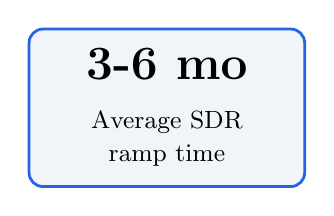
\begin{tikzpicture}
\node[draw=sparrowblue, line width=1pt, rounded corners=5pt, fill=sparrowlight, minimum width=3.5cm, minimum height=2cm, align=center] {
    {\LARGE\textbf{3-6 mo}}\\[0.2cm]
    {\small Average SDR}\\
    {\small ramp time}
};
\end{tikzpicture}
&
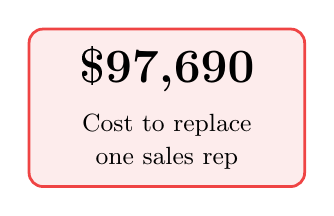
\begin{tikzpicture}
\node[draw=sparrowred, line width=1pt, rounded corners=5pt, fill=sparrowred!10, minimum width=3.5cm, minimum height=2cm, align=center] {
    {\LARGE\textbf{\$97,690}}\\[0.2cm]
    {\small Cost to replace}\\
    {\small one sales rep}
};
\end{tikzpicture}
&
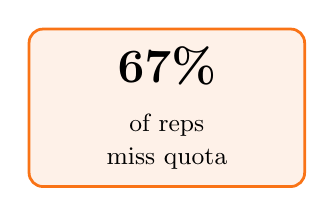
\begin{tikzpicture}
\node[draw=sparroworange, line width=1pt, rounded corners=5pt, fill=sparroworange!10, minimum width=3.5cm, minimum height=2cm, align=center] {
    {\LARGE\textbf{67\%}}\\[0.2cm]
    {\small of reps}\\
    {\small miss quota}
};
\end{tikzpicture}
\end{tabular}
\end{center}

\vspace{0.3cm}

\begin{center}
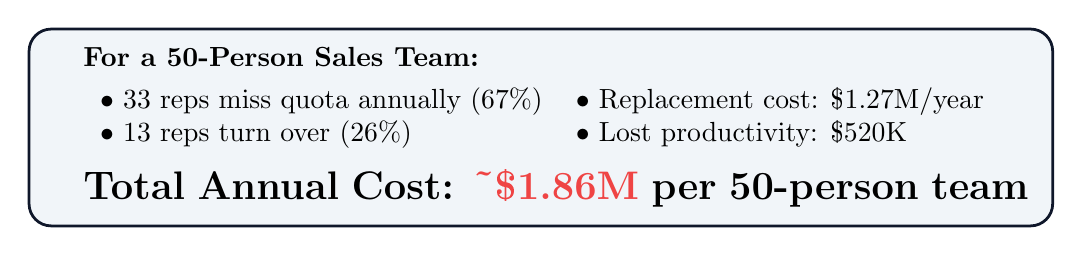
\begin{tikzpicture}
\node[draw=sparrowdark, line width=1pt, rounded corners=8pt, fill=sparrowlight, minimum width=13cm, minimum height=2.5cm, align=left] {
\hspace{0.5cm}\begin{minipage}{12cm}
\textbf{For a 50-Person Sales Team:}\\[0.2cm]
\begin{tabular}{ll}
$\bullet$ 33 reps miss quota annually (67\%) & $\bullet$ Replacement cost: \$1.27M/year\\
$\bullet$ 13 reps turn over (26\%) & $\bullet$ Lost productivity: \$520K\\
\end{tabular}\\[0.2cm]
{\Large\textbf{Total Annual Cost: \textcolor{sparrowred}{\textasciitilde\$1.86M} per 50-person team}}
\end{minipage}
};
\end{tikzpicture}
\end{center}

\end{frame}

% ==================== SLIDE 4: THE SOLUTION ====================
\begin{frame}
\frametitle{\textbf{The Solution}}
\framesubtitle{Sparrow: Your AI Sales Sparring Partner}

\begin{center}
{\Large\textbf{\textcolor{sparrowblue}{Practice sales conversations with AI that pushes back like real buyers}}}
\end{center}

\vspace{0.5cm}

\begin{columns}[T]
\begin{column}{0.55\textwidth}
\textbf{How It Works:}\\[0.4cm]

\textcolor{sparrowblue}{1.} \textbf{Choose Your Scenario}\\
{\small Cold call, Discovery, or Objection Gauntlet}\\[0.3cm]

\textcolor{sparrowblue}{2.} \textbf{Meet Your AI Prospect}\\
{\small Realistic backstory, pain points, objections}\\
{\small\textcolor{sparrowgray}{``Sarah Chen, VP Ops at LogiFlow''}}\\[0.3cm]

\textcolor{sparrowblue}{3.} \textbf{Have a Real Conversation}\\
{\small Speak naturally --- AI responds with voice}\\
{\small\textcolor{sparrowgray}{``We're not looking at new solutions...''}}\\[0.3cm]

\textcolor{sparrowblue}{4.} \textbf{Get Instant Feedback}\\
{\small Scored across 5 dimensions}\\
{\small\textcolor{sparrowgray}{``At 1:12, you missed an opportunity...''}}
\end{column}
\begin{column}{0.42\textwidth}
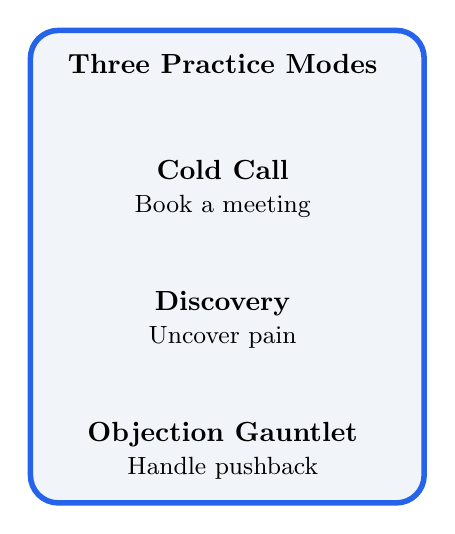
\begin{tikzpicture}
\node[draw=sparrowblue, line width=2pt, rounded corners=10pt, fill=sparrowlight, minimum width=5cm, minimum height=6cm, align=center] {
\begin{minipage}{4.5cm}
\centering
\textbf{Three Practice Modes}\\[0.5cm]
\textcolor{sparrowblue}{\Large$\phone$}\\
\textbf{Cold Call}\\
{\small Book a meeting}\\[0.4cm]
\textcolor{sparrowgreen}{\Large$\varnothing$}\\
\textbf{Discovery}\\
{\small Uncover pain}\\[0.4cm]
\textcolor{sparroworange}{\Large$\lightning$}\\
\textbf{Objection Gauntlet}\\
{\small Handle pushback}
\end{minipage}
};
\end{tikzpicture}
\end{column}
\end{columns}

\end{frame}

% ==================== SLIDE 5: PRODUCT DEMO ====================
\begin{frame}
\frametitle{\textbf{Product Demo}}
\framesubtitle{The Sparrow Experience}

\begin{columns}[T]
\begin{column}{0.32\textwidth}
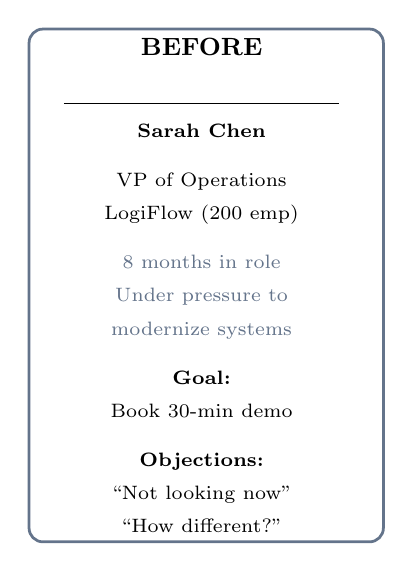
\begin{tikzpicture}
\node[draw=sparrowgray, line width=1pt, rounded corners=5pt, fill=white, minimum width=4.5cm, minimum height=4.5cm, align=left] {
\begin{minipage}{4cm}
\centering
\textbf{\small BEFORE}\\[0.2cm]
\rule{3.5cm}{0.4pt}
\vspace{0.2cm}
{\scriptsize \textbf{Sarah Chen}}\\
{\scriptsize VP of Operations}\\
{\scriptsize LogiFlow (200 emp)}\\[0.2cm]
{\scriptsize\textcolor{sparrowgray}{8 months in role}}\\
{\scriptsize\textcolor{sparrowgray}{Under pressure to}}\\
{\scriptsize\textcolor{sparrowgray}{modernize systems}}\\[0.2cm]
{\scriptsize \textbf{Goal:}}\\
{\scriptsize Book 30-min demo}\\[0.2cm]
{\scriptsize \textbf{Objections:}}\\
{\scriptsize ``Not looking now''}\\
{\scriptsize ``How different?''}
\end{minipage}
};
\end{tikzpicture}
\end{column}
\begin{column}{0.32\textwidth}
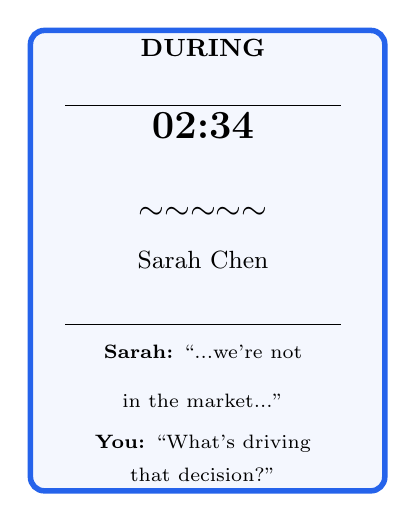
\begin{tikzpicture}
\node[draw=sparrowblue, line width=2pt, rounded corners=5pt, fill=sparrowblue!5, minimum width=4.5cm, minimum height=4.5cm, align=center] {
\begin{minipage}{4cm}
\centering
\textbf{\small DURING}\\[0.2cm]
\rule{3.5cm}{0.4pt}
\vspace{0.3cm}
{\Large \textbf{02:34}}\\[0.3cm]
{\large $\sim\sim\sim\sim\sim$}\\[0.2cm]
{\small Sarah Chen}\\[0.3cm]
\rule{3.5cm}{0.4pt}
\vspace{0.2cm}
{\scriptsize\textbf{Sarah:} ``...we're not}\\
{\scriptsize in the market...''}\\[0.1cm]
{\scriptsize\textbf{You:} ``What's driving}\\
{\scriptsize that decision?''}
\end{minipage}
};
\end{tikzpicture}
\end{column}
\begin{column}{0.32\textwidth}
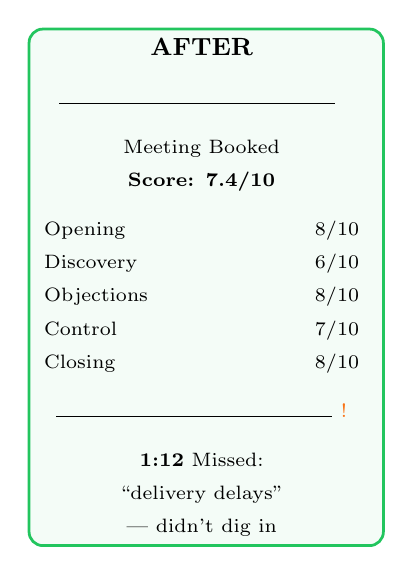
\begin{tikzpicture}
\node[draw=sparrowgreen, line width=1pt, rounded corners=5pt, fill=sparrowgreen!5, minimum width=4.5cm, minimum height=4.5cm, align=left] {
\begin{minipage}{4cm}
\centering
\textbf{\small AFTER}\\[0.2cm]
\rule{3.5cm}{0.4pt}
\vspace{0.2cm}
{\scriptsize\textcolor{sparrowgreen}{$\checkmark$} Meeting Booked}\\
{\scriptsize\textbf{Score: 7.4/10}}\\[0.2cm]
{\scriptsize Opening \hfill 8/10}\\
{\scriptsize Discovery \hfill 6/10}\\
{\scriptsize Objections \hfill 8/10}\\
{\scriptsize Control \hfill 7/10}\\
{\scriptsize Closing \hfill 8/10}\\[0.2cm]
\rule{3.5cm}{0.4pt}
\vspace{0.2cm}
{\scriptsize\textcolor{sparroworange}{!} \textbf{1:12} Missed:}\\
{\scriptsize ``delivery delays''}\\
{\scriptsize --- didn't dig in}
\end{minipage}
};
\end{tikzpicture}
\end{column}
\end{columns}

\vspace{0.5cm}

\begin{center}
{\large\textbf{Result: Reps practice 10-20 calls/day instead of 0}}
\end{center}

\end{frame}

% ==================== SLIDE 6: TECHNOLOGY ====================
\begin{frame}
\frametitle{\textbf{Technology \& Differentiation}}
\framesubtitle{Powered by Best-in-Class AI}

\begin{columns}[T]
\begin{column}{0.5\textwidth}
\textbf{Technology Stack:}\\[0.4cm]

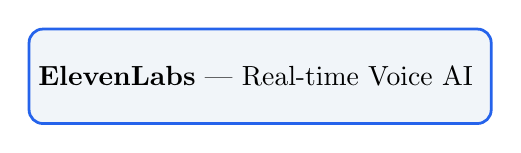
\begin{tikzpicture}
\node[draw=sparrowblue, line width=1pt, rounded corners=5pt, fill=sparrowlight, minimum width=5.5cm, minimum height=1.2cm, align=center] {
\textbf{ElevenLabs} --- Real-time Voice AI
};
\end{tikzpicture}\\[0.3cm]


\begin{tikzpicture}
\node[draw=sparrowblue, line width=1pt, rounded corners=5pt, fill=sparrowlight, minimum width=5.5cm, minimum height=1.2cm, align=center] {
\textbf{Google Gemini} --- Persona \& Analysis
};
\end{tikzpicture}\\[0.3cm]

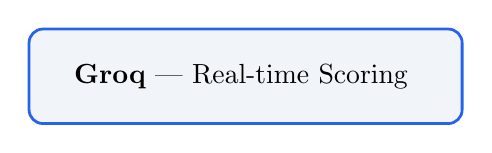
\begin{tikzpicture}
\node[draw=sparrowblue, line width=1pt, rounded corners=5pt, fill=sparrowlight, minimum width=5.5cm, minimum height=1.2cm, align=center] {
\textbf{Groq} --- Real-time Scoring
};
\end{tikzpicture}\\[0.3cm]

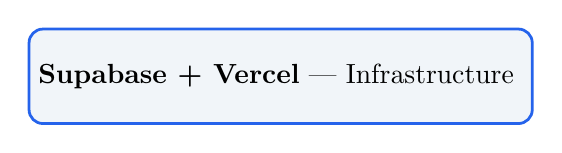
\begin{tikzpicture}
\node[draw=sparrowblue, line width=1pt, rounded corners=5pt, fill=sparrowlight, minimum width=5.5cm, minimum height=1.2cm, align=center] {
\textbf{Supabase + Vercel} --- Infrastructure
};
\end{tikzpicture}

\end{column}
\begin{column}{0.48\textwidth}
\textbf{What Makes Sparrow Different:}\\[0.4cm]

\begin{tabular}{p{2.5cm}|p{3cm}}
\textbf{\small Traditional} & \textbf{\small Sparrow}\\
\hline
{\scriptsize Read a book} & {\scriptsize Practice out loud}\\
{\scriptsize Watch video} & {\scriptsize Real-time pushback}\\
{\scriptsize Roleplay w/ mgr} & {\scriptsize AI like real buyers}\\
{\scriptsize ``That was good''} & {\scriptsize Timestamped feedback}\\
{\scriptsize Real prospects} & {\scriptsize Safe to fail}\\
{\scriptsize Work hours} & {\scriptsize Available 24/7}\\
\end{tabular}

\vspace{0.5cm}

\textbf{Advantages:}\\[0.2cm]
{\small$\checkmark$ Voice-first (not chatbots)}\\
{\small$\checkmark$ Dynamic personas}\\
{\small$\checkmark$ Objective scoring}\\
{\small$\checkmark$ Adaptive difficulty}

\end{column}
\end{columns}

\end{frame}

% ==================== SLIDE 7: MARKET OPPORTUNITY ====================
\begin{frame}
\frametitle{\textbf{Market Opportunity}}
\framesubtitle{Clear TAM $\rightarrow$ SAM $\rightarrow$ SOM with Calculations}

\begin{columns}[T]
\begin{column}{0.58\textwidth}

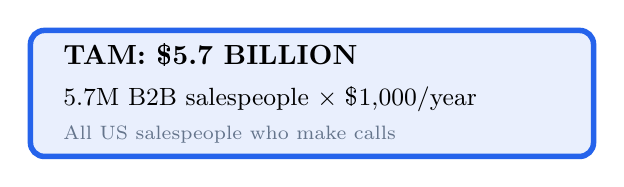
\begin{tikzpicture}
\node[draw=sparrowblue, line width=2pt, rounded corners=5pt, fill=sparrowblue!10, minimum width=7cm, minimum height=1.6cm, align=left] {
\hspace{0.3cm}\begin{minipage}{6.5cm}
\textbf{TAM: \$5.7 BILLION}\\[0.1cm]
{\small 5.7M B2B salespeople $\times$ \$1,000/year}\\
{\scriptsize\textcolor{sparrowgray}{All US salespeople who make calls}}
\end{minipage}
};
\end{tikzpicture}

\vspace{0.2cm}

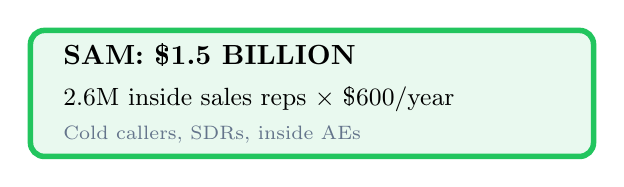
\begin{tikzpicture}
\node[draw=sparrowgreen, line width=2pt, rounded corners=5pt, fill=sparrowgreen!10, minimum width=7cm, minimum height=1.6cm, align=left] {
\hspace{0.3cm}\begin{minipage}{6.5cm}
\textbf{SAM: \$1.5 BILLION}\\[0.1cm]
{\small 2.6M inside sales reps $\times$ \$600/year}\\
{\scriptsize\textcolor{sparrowgray}{Cold callers, SDRs, inside AEs}}
\end{minipage}
};
\end{tikzpicture}

\vspace{0.2cm}

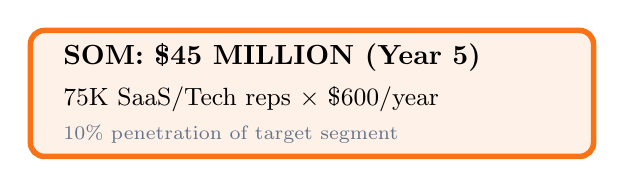
\begin{tikzpicture}
\node[draw=sparroworange, line width=2pt, rounded corners=5pt, fill=sparroworange!10, minimum width=7cm, minimum height=1.6cm, align=left] {
\hspace{0.3cm}\begin{minipage}{6.5cm}
\textbf{SOM: \$45 MILLION (Year 5)}\\[0.1cm]
{\small 75K SaaS/Tech reps $\times$ \$600/year}\\
{\scriptsize\textcolor{sparrowgray}{10\% penetration of target segment}}
\end{minipage}
};
\end{tikzpicture}

\end{column}
\begin{column}{0.4\textwidth}

\textbf{Year-by-Year Path:}\\[0.3cm]

\begin{tabular}{lrl}
\textbf{Yr 1} & 1K users & \$600K\\
\textbf{Yr 2} & 5K users & \$3M\\
\textbf{Yr 3} & 15K users & \$9M\\
\textbf{Yr 4} & 35K users & \$21M\\
\textbf{Yr 5} & 75K users & \$45M\\
\end{tabular}

\vspace{0.5cm}

\textbf{Why Now:}\\[0.2cm]
{\small$\checkmark$ Voice AI ready (2024)}\\
{\small$\checkmark$ 91\% miss quota}\\
{\small$\checkmark$ Remote sales growth}\\
{\small$\checkmark$ \$2K/rep budget exists}

\end{column}
\end{columns}

\vspace{0.2cm}

\begin{center}
{\small\textcolor{sparrowgray}{Sources: BLS, US Census, HubSpot, QuotaPath}}
\end{center}

\end{frame}

% ==================== SLIDE 8: BUSINESS MODEL ====================
\begin{frame}
\frametitle{\textbf{Business Model}}
\framesubtitle{Simple, Scalable Revenue Model}

\begin{columns}[T]
\begin{column}{0.55\textwidth}
\textbf{Pricing Tiers:}\\[0.3cm]

\begin{tabular}{ccc}
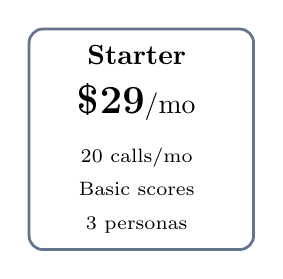
\begin{tikzpicture}
\node[draw=sparrowgray, line width=1pt, rounded corners=5pt, fill=white, minimum width=2.8cm, minimum height=2.8cm, align=center] {
\begin{minipage}{2.5cm}
\centering
\textbf{Starter}\\[0.2cm]
{\Large\textbf{\$29}}/mo\\[0.2cm]
{\scriptsize 20 calls/mo}\\
{\scriptsize Basic scores}\\
{\scriptsize 3 personas}
\end{minipage}
};
\end{tikzpicture}
&
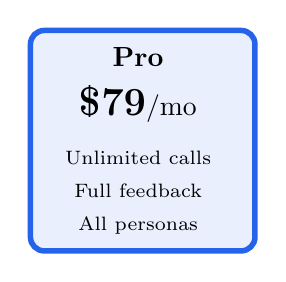
\begin{tikzpicture}
\node[draw=sparrowblue, line width=2pt, rounded corners=5pt, fill=sparrowblue!10, minimum width=2.8cm, minimum height=2.8cm, align=center] {
\begin{minipage}{2.5cm}
\centering
\textbf{Pro}\\[0.2cm]
{\Large\textbf{\$79}}/mo\\[0.2cm]
{\scriptsize Unlimited calls}\\
{\scriptsize Full feedback}\\
{\scriptsize All personas}
\end{minipage}
};
\end{tikzpicture}
&
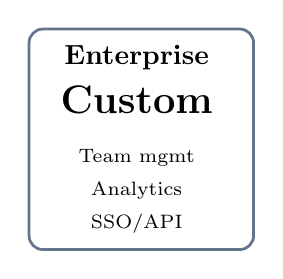
\begin{tikzpicture}
\node[draw=sparrowgray, line width=1pt, rounded corners=5pt, fill=white, minimum width=2.8cm, minimum height=2.8cm, align=center] {
\begin{minipage}{2.5cm}
\centering
\textbf{Enterprise}\\[0.2cm]
{\Large\textbf{Custom}}\\[0.2cm]
{\scriptsize Team mgmt}\\
{\scriptsize Analytics}\\
{\scriptsize SSO/API}
\end{minipage}
};
\end{tikzpicture}
\end{tabular}

\end{column}
\begin{column}{0.43\textwidth}

\textbf{Unit Economics:}\\[0.3cm]

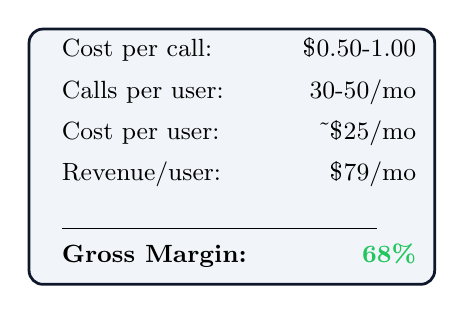
\begin{tikzpicture}
\node[draw=sparrowdark, line width=1pt, rounded corners=5pt, fill=sparrowlight, minimum width=5cm, minimum height=3.2cm, align=left] {
\hspace{0.3cm}\begin{minipage}{4.5cm}
{\small Cost per call:} \hfill {\small \$0.50-1.00}\\[0.1cm]
{\small Calls per user:} \hfill {\small 30-50/mo}\\[0.1cm]
{\small Cost per user:} \hfill {\small \textasciitilde\$25/mo}\\[0.1cm]
{\small Revenue/user:} \hfill {\small \$79/mo}\\[0.2cm]
\rule{4cm}{0.4pt}
\vspace{0.1cm}
{\small\textbf{Gross Margin:}} \hfill {\small\textbf{\textcolor{sparrowgreen}{68\%}}}
\end{minipage}
};
\end{tikzpicture}

\vspace{0.3cm}

\textbf{ARPU:} \$600/year (blended)

\end{column}
\end{columns}

\end{frame}

% ==================== SLIDE 9: TRACTION & ROADMAP ====================
\begin{frame}
\frametitle{\textbf{Traction \& Roadmap}}
\framesubtitle{Current Status \& Next Steps}

\begin{columns}[T]
\begin{column}{0.48\textwidth}
\textbf{Current Status (MVP):}\\[0.3cm]

\textcolor{sparrowgreen}{$\checkmark$} Working voice AI (ElevenLabs)\\[0.15cm]
\textcolor{sparrowgreen}{$\checkmark$} Dynamic personas (Gemini)\\[0.15cm]
\textcolor{sparrowgreen}{$\checkmark$} Real-time scoring (Groq)\\[0.15cm]
\textcolor{sparrowgreen}{$\checkmark$} 3 practice modes\\[0.15cm]
\textcolor{sparrowgreen}{$\checkmark$} Post-call debrief\\[0.15cm]
\textcolor{sparrowgreen}{$\checkmark$} User auth \& dashboard\\[0.15cm]
\textcolor{sparrowgreen}{$\checkmark$} Deployed on Vercel\\[0.3cm]

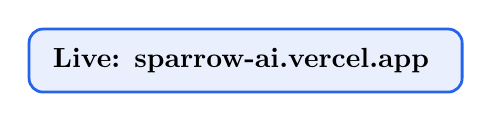
\begin{tikzpicture}
\node[draw=sparrowblue, line width=1pt, rounded corners=5pt, fill=sparrowblue!10, minimum width=5.5cm, minimum height=0.8cm, align=center] {
\textbf{Live: sparrow-ai.vercel.app}
};
\end{tikzpicture}

\end{column}
\begin{column}{0.5\textwidth}
\textbf{Roadmap:}\\[0.3cm]

\begin{tabular}{p{2.3cm}|p{2.8cm}}
\textbf{Q1 2025} & \textbf{Q2 2025}\\
\hline
{\scriptsize Public launch} & {\scriptsize Team dashboard}\\
{\scriptsize Stripe billing} & {\scriptsize Custom personas}\\
{\scriptsize 10+ templates} & {\scriptsize Recording playback}\\
{\scriptsize Mobile UI} & {\scriptsize Leaderboards}\\
\end{tabular}

\vspace{0.3cm}

\begin{tabular}{p{2.3cm}|p{2.8cm}}
\textbf{Q3 2025} & \textbf{Q4 2025}\\
\hline
{\scriptsize Enterprise SSO} & {\scriptsize CRM integrations}\\
{\scriptsize API access} & {\scriptsize AI coaching}\\
{\scriptsize Multi-language} & {\scriptsize Library sharing}\\
{\scriptsize Analytics} & {\scriptsize White-label}\\
\end{tabular}

\end{column}
\end{columns}

\end{frame}

% ==================== SLIDE 10: THE ASK ====================
{
\setbeamertemplate{footline}{}
\begin{frame}
\begin{center}
\vspace{0.5cm}

{\Huge\textbf{\textcolor{sparrowblue}{SPARROW}}}

\vspace{0.3cm}

{\Large ``Never Wing a Call Again''}

\vspace{0.6cm}


\begin{tikzpicture}
\draw[sparrowblue, line width=2pt] (0,0) -- (10,0);
\end{tikzpicture}

\vspace{0.5cm}

\begin{columns}[T]
\begin{column}{0.48\textwidth}
\textbf{The Opportunity:}\\[0.3cm]
{\small$\checkmark$ \$5.7B TAM, 13-15\% CAGR}\\[0.15cm]
{\small$\checkmark$ 91\% miss quota}\\[0.15cm]
{\small$\checkmark$ Voice AI finally ready}\\[0.15cm]
{\small$\checkmark$ Path to \$45M ARR (Yr 5)}
\end{column}
\begin{column}{0.48\textwidth}
\textbf{Why Sparrow Wins:}\\[0.3cm]
{\small$\checkmark$ Voice-first (not chatbots)}\\[0.15cm]
{\small$\checkmark$ Realistic AI prospects}\\[0.15cm]
{\small$\checkmark$ Objective scoring}\\[0.15cm]
{\small$\checkmark$ Available 24/7}
\end{column}
\end{columns}

\vspace{0.6cm}


\begin{tikzpicture}
\draw[sparrowblue, line width=2pt] (0,0) -- (10,0);
\end{tikzpicture}

\vspace{0.5cm}

{\LARGE\textbf{Try It Now}}

\vspace{0.3cm}


\begin{tikzpicture}
\node[draw=sparrowblue, line width=2pt, rounded corners=10pt, fill=sparrowblue, minimum width=6cm, minimum height=1cm, align=center] {
{\large\textcolor{white}{\textbf{sparrow-ai.vercel.app}}}
};
\end{tikzpicture}

\end{center}
\end{frame}
}

\end{document}
